
 
\section{Scenegraph}

\begin{frame}
\tableofcontents[currentsection]
\end{frame}
 
 
\subsection{Einleitung}
\frame %%Eine Folie
{
  \frametitle{Was ist der Scenegraph?} %%Folientitel
	  \begin{itemize}
	  \item Baum, der aus verschiedenen Knoten besteht
	  \item hält alle Informationen die zum Rendern benötigt werden
	  \item Root-Knoten ist als $<$0;0;0$>$ definiert und hat keine Rotation
	  \item Innere Knoten beinhalten Transformationsmatrizen
	  \item Blätter beinhalten die zu rendernden Objekte (ihre Texturen)
	  \item Position und Rotation der Objekte wird durch Multiplikation der Matrizen vom root bis zum jeweiligen Blatt berechnet
	\end{itemize}
}

\subsection{Aufbau}
\frame
{
  \frametitle{Wie ist der Scenegraph aufgebaut?} %%Folientitel
	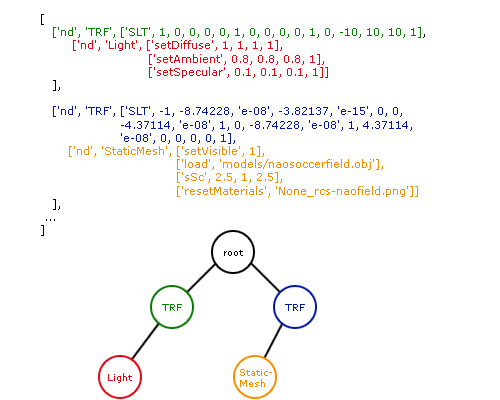
\includegraphics[width=0.8\textwidth]{Scene}
}

\subsection{Nutzen}
\frame %%Eine Folie
{
  \frametitle{Wozu brauchen wir den Scenegraph?} %%Folientitel
  	 \begin{itemize}
	  \item Auslesen der exakten Position eines Objekts (z.B. unseres NAOs)
	  \item Analyse unseres Teams und des Gegners
	\end{itemize}
}

\subsection{Problemstellungen}
\frame
{
  \frametitle{Problemstellungen (TODO)} %%Folientitel
	 Wir wissen noch nicht in welcher Reihenfolge die NAOs im Scenegraph gespeichert werden. Da die IDs der NAOs nicht mit "ubertragen werden, m"ussen wir testen, wie wir die NAOs im Scenegraph identifizieren k"onnen.
}